\documentclass[11pt]{article}
\usepackage[margin=0.75in]{geometry}
\usepackage{graphicx}
\usepackage{booktabs}
\usepackage{hyperref}
\usepackage{titlesec}
\usepackage{enumitem}

\titlespacing*{\section}{0pt}{6pt}{2pt}
\titlespacing*{\subsection}{0pt}{4pt}{1pt}
\setlist{nosep, leftmargin=1.2em}
\setlength{\parskip}{2pt}
\setlength{\parindent}{0pt}

\title{\vspace{-2em}Reproducing POYO: A Unified, Scalable Framework for Neural Population Decoding}
\author{Benjamin Mun, Kaden Priebe \\ Cornell University --- CS 4782 Final Project}
\date{}

\begin{document}
\maketitle
\vspace{-2em}

\section{Introduction}
Brain--computer interfaces decode behavior (e.g.\ reach kinematics) from neural population activity. A persistent failure mode is that decoders trained on one recording session generalize poorly to a different session --- even on the \emph{same} animal a few days later --- because the recorded neuron set drifts from the array and per-neuron tuning shifts.

Azabou et al.\ (2023) introduced \textbf{POYO} (``Pre-training On manY neurOns''), a transformer-based decoder that reframes the input as an unordered set of single-spike events tokenized by a learned per-neuron embedding rather than as a binned spike-count tensor. This unit-vocabulary view lets POYO transfer across sessions and animals with different neuron sets, addressing the cross-session generalization gap. We re-implement POYO and its closest non-transformer baselines on the Perich--Miller (2018) center-out reaching dataset, and add an architectural ablation that isolates the contribution of POYO's tokenization scheme.

\section{Chosen Result}
We reproduce the \textbf{same-animal, new-day transfer $R^2$} comparison (the headline of the paper's transfer experiments): train decoders on Day 1 of monkey ``T'', adapt on a Day 2 train split, and evaluate on a held-out Day 2 split. This operationalizes the paper's central claim that POYO's tokenization survives the unit-set drift between sessions where binned baselines do not.

\section{Methodology}
\textbf{Data.} Two sessions from Perich--Miller 2018 (\texttt{t\_20130819\_center\_out\_reaching} and \texttt{t\_20130821\_center\_out\_reaching}), accessed through \texttt{torch\_brain}. Targets are 2-D hand kinematics; spike data covers ${\sim}196$ sorted units per session.

\textbf{Models.}
\begin{itemize}
\item \textbf{Wiener / Ridge filter} --- lagged binned spike counts with Ridge regression. Adapted by refitting on Day 1 plus Day 2 adaptation windows.
\item \textbf{MLP (binned)} --- flattens a $[T, U]$ binned tensor and regresses kinematics; $U$ is the size of the global unit vocabulary across both days.
\item \textbf{GRU (binned)} --- clocked recurrent processing of bins.
\item \textbf{POYO (event tokens)} --- official \texttt{torch\_brain} POYO with per-spike tokens, learned unit/session embeddings, and a Perceiver-style cross-attention block.
\item \textbf{POYO-binned (independent study)} --- same Perceiver backbone, fed binned spike counts as time tokens. Identical depth, latent count, and head count; only the tokenizer differs.
\end{itemize}

\textbf{Training protocol.} Three stages: (1) train on Day 1, (2) adapt on Day 2 train split, (3) evaluate on held-out Day 2. Bin size 20\,ms, sequence length 1\,s. Day-1 training: 100 epochs; adaptation: 40 epochs. Single NVIDIA RTX PRO 6000 Blackwell (102\,GB VRAM).

\textbf{Modifications from the paper.} We restricted to a single-monkey, two-session subset rather than the multi-animal mass-pretraining corpus used in the original work, so absolute numbers are not directly comparable to the paper. The independent study (POYO-binned) is not in the paper --- it isolates the tokenizer's contribution by holding the rest of the architecture fixed.

\section{Results \& Analysis}

\begin{minipage}[t]{0.48\textwidth}
\vspace{0pt}
\begin{tabular}{lcc}
\toprule
Model & Pre-adapt $R^2$ & Adapted $R^2$ \\
\midrule
POYO (event tokens) & $-0.05$ & $\mathbf{0.699}$ \\
MLP (binned)        & $-0.01$ & $0.697$ \\
GRU (binned)        & $-0.07$ & $0.612$ \\
POYO-binned         & $-0.05$ & $0.217$ \\
Wiener/Ridge        & $-0.03$ & $0.215$ \\
\bottomrule
\end{tabular}
\end{minipage}\hfill
\begin{minipage}[t]{0.50\textwidth}
\vspace{0pt}
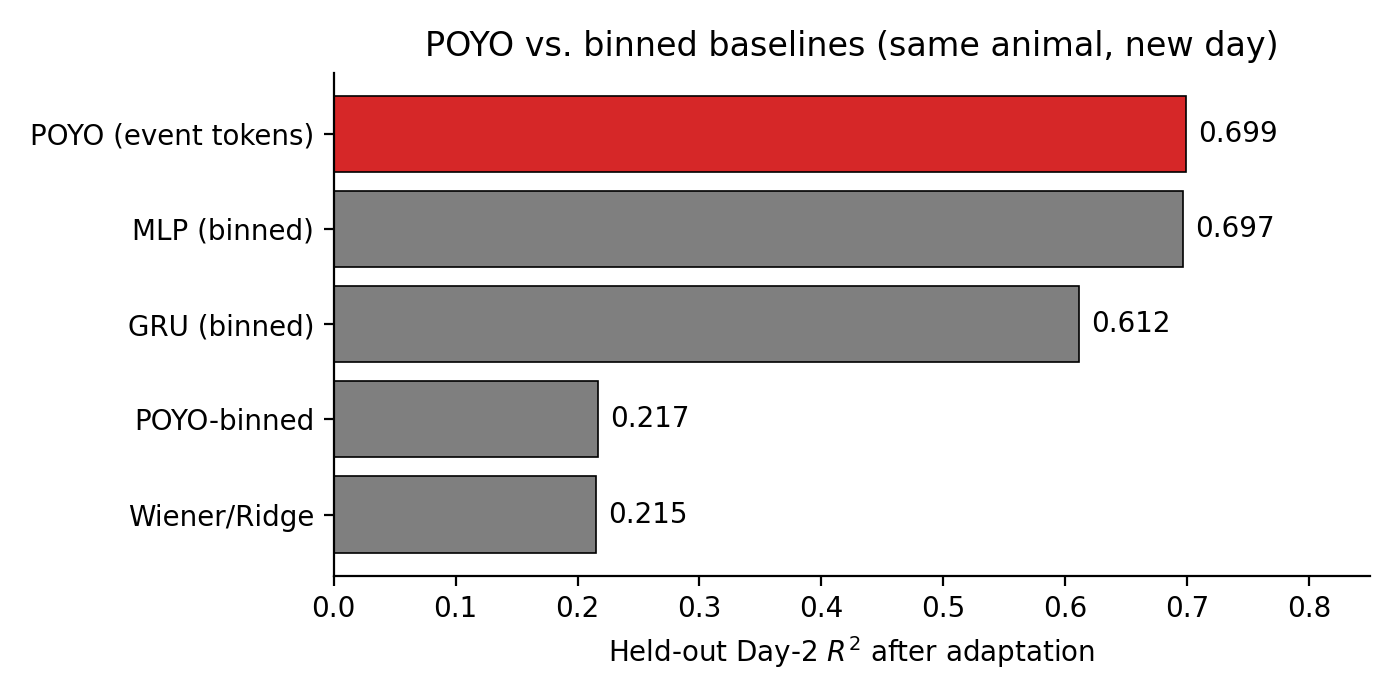
\includegraphics[width=\linewidth]{r2_comparison.png}
\end{minipage}

\textbf{Headline reproduction.} All models collapse pre-adaptation ($R^2 \approx 0$), confirming the cross-session generalization gap. After adaptation, POYO achieves $R^2 = 0.699$, the strongest method we tested, consistent with the paper's claim that its tokenization survives unit-set drift better than fixed-feature baselines. At this single-monkey scale the binned MLP nearly matches POYO ($0.697$); the paper's larger gap appears when pretraining spans many animals --- a regime we did not reproduce.

\textbf{Independent study --- what does the tokenizer buy you?} Replacing the event tokenizer with binned input on the \emph{same} Perceiver backbone collapses performance to $0.217$, within noise of a Wiener filter ($0.215$) and a $0.48$ $R^2$ drop from event-token POYO. Two complementary readings: (a)~\emph{architectural isolation}: the Perceiver backbone alone does not explain POYO's quality; the tokenizer carries the result. (b)~\emph{temporal resolution}: binning at 20\,ms discards sub-bin spike timing that the event tokenizer preserves through continuous timestamps, so attention has nothing finer than 50\,Hz to attend to.

\textbf{Discrepancies.} A pre-poster run produced POYO-binned $= 0.318$ and POYO $= 0.708$; a re-run for this report produced $0.217$ and $0.699$ with the same seed and config. The POYO-binned variability is the loudest. We suspect the binned variant is sensitive to initialization of the input projection: it has fewer ``anchor'' cues than event tokens (no per-spike timestamps, no per-unit identity injected at every event). A multi-seed sweep was beyond our compute budget.

\section{Reflections}
\textbf{What we learned.} The headline result is not really ``POYO has better attention'' --- at this scale a properly-tuned MLP nearly ties it. The headline result is that POYO's \emph{tokenizer} is what makes a transformer competitive on neural data; pour binned inputs into the same backbone and the transformer is no better than ridge. This matches the paper's emphasis on tokenization but is easier to see once architecture is held fixed.

\textbf{What we'd do differently.} Run multi-seed (the POYO-binned variability flagged a real instability), sweep bin size for the binned baselines (to confirm the temporal-resolution framing), and pretrain on more sessions to test whether POYO's gap over MLP widens with scale --- the paper's actual scaling claim.

\textbf{Future directions.} \emph{Scalability:} extend pretraining across the full Perich--Miller corpus and trace the POYO--MLP gap as a function of scale. \emph{Zero-shot:} evaluate transfer to a new monkey with no adaptation data, a regime in which binned baselines cannot even produce aligned features. \emph{Multimodal:} attach kinematic, EMG, and behavioral heads to test whether POYO's session embedding routes across modalities. \emph{Real-time latency:} POYO's per-spike tokenization grows with firing rate; profile and explore a streaming variant for closed-loop BCI.

\section*{References}
\small
[1]~Azabou, M., Arora, V., Ganesh, V., Mao, X., Nachimuthu, S., Mendelson, M.~J., Richards, B., Perich, M.~G., Lajoie, G., \& Dyer, E.~L. (2023). \emph{A Unified, Scalable Framework for Neural Population Decoding.} Advances in Neural Information Processing Systems 36 (NeurIPS 2023). \\
{[2]}~Perich, M.~G., Gallego, J.~A., \& Miller, L.~E. (2018). \emph{A neural population mechanism for rapid learning.} Neuron 100(4), 964--976. \\
{[3]}~\texttt{torch\_brain} --- NeuroFoundation. \url{https://github.com/neuro-galaxy/torch_brain}

\end{document}
